\section{HW/SW Co-Design}
Ziel von HW/SW Co-Design ist es den Entwurf, so lange wie sinvoll, lösungsneutral zu erarbeiten und dadurch Implementationen einfach ändern von HW zu SW und umgekehrt.

Oft werden diese Entwürfe mittels \textbf{x-in-the-loop} getestet. Dabei wird schritt für schritt der Prototype durch eine konkrete Implementierung ersetzt. Bei start ist oft nur ein virtuelles Modell verfügbar, welches durch Model-in-the-Loop (MIL) ausgewürt werden kann.
\begin{center}
	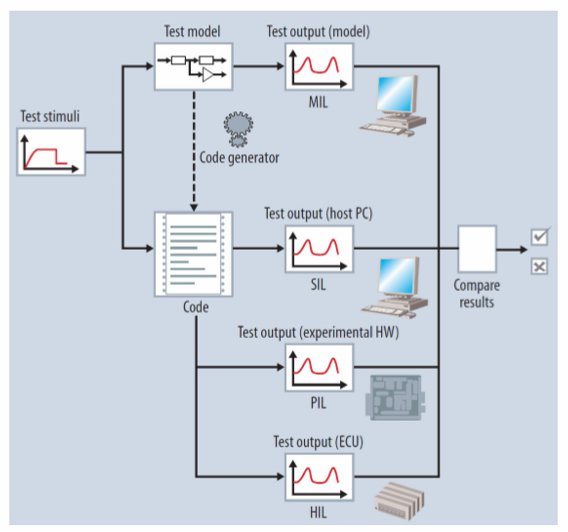
\includegraphics[width=\columnwidth]{Images/model-in-the-loop}
\end{center}
